\chapter{Bài Toán Tối Ưu Tổ Hợp}
\label{chap:combOpt}
%======================================================================
\section{Tổ hợp và không gian tìm kiếm}
\label{sec:co_space}

%-----------------------------------------------------------------
\subsection{Khái niệm}

\subsubsection*{Bài Toán Tối ưu tổ hợp}
Bài toán tối ưu tổ hợp \cite{pascal2005cp} là một dạng của bài toán tối ưu, nó có dạng tổng quát như sau:
\begin{itemize}
	\item Cho hàm $f(X)$ xác định trên một tập hữu hạn các phần tử $D$, hàm $f(x)$ được gọi là hàm mục tiêu.
	\item Mỗi phần tử $X$ thuộc $D$ có dạng $X=(x_1,\dots,x_n)$ được gọi là một phương án.
	\item Cần tìm một phương án $X$ thuộc $D$ sao cho hàm $f(X)$ đạt cực tiểu, phương án $X$ như vậy được gọi là phương án tối ưu.
\end{itemize}

\subsubsection*{Bài toán thỏa mãn ràng buộc}

Bài toán thỏa mãn ràng buộc \cite{pascal2005cp} là bài toán tối ưu tổ hợp bổ sung thêm các điều kiện ràng buộc được xác định bởi bộ
\[
\{X, D, C, F\}
\]
với:
\begin{description}
	\item $X = \{X_1,\dotsc, X_n\}$ \quad là tập các biến.
	\item $D = \{D_1,\dotsc, D_n\}$ \quad là tập miền xác định tương ứng của các biến.
	\item $C = \{C_1,\dotsc, C_m\}$ \quad là tập các ràng buộc.
	\item $F = \{F_1,\dotsc, F_k\}$ \quad là tập các hàm mục tiêu cần tối ưu.
\end{description}

Tập $S = \{t_1,\dotsc, t_n\}$ với phần tử $t_i$ là giá trị tương ứng của mỗi biến $X_i$ và $S$ thỏa mãn tất cả các ràng buộc định nghĩa trong $C$ thì $S$ được gọi là tập lời giải của bài toán thỏa mãn ràng buộc trên bộ $\{X, D, C\}$.

Trong nhiều bài toán chúng ta còn cần phải tối ưu thêm các mục tiêu:
\begin{equation}
F_i = f(X_1,\dotsc, X_n) \quad 1 \leq i \leq k.
\end{equation}
Lời giải $S^*$ trong tập các lời giải $S$ của bài toán thỏa mãn ràng buộc trên đồng thời cho giá trị cực tiểu của các hàm mục tiêu $F_i$ thì $S^*$ được gọi là lời giải tối ưu của bài toán.

\subsubsection*{Không gian tìm kiếm lời giải}
Tất cả các bài toán tối ưu tổ hợp đều có độ phức tạp tính toán hàm mũ, chúng thuộc lớp các bài toán \textsf{NP-khó} và chưa có các thuật toán hiệu quả để tìm kiếm lời giải.

%------------------------------------------------------------------
\subsection{Ví dụ}

\subsubsection*{N-QUEEN}

\begin{figure}
	\centering
	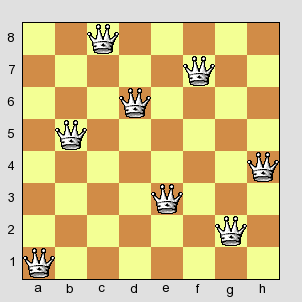
\includegraphics[scale=1]{figures/10-queens-sol.png}
	\caption{Lời giải của bài toán 8 con hậu \cite{PaulButler2009queens}.\label{fig:queens}}
\end{figure}

Bài toán sắp xếp $N ( N > 4)$ quân hậu yêu cầu sắp xếp $N$ quân hậu trên bàn cờ vua sao cho không có quân hậu nào có thể \textsc{ăn} được các quân hậu còn lại theo quy tắc cờ vua. Hay có thể phát biểu rằng không có hai con hậu nào cùng nằm tren một hàng, một cột hoặc một đường chéo.

Mô hình toán học:
\begin{list}{•}{}
	\item $X = \{x_i | 1 \le i \le N \}$ \quad với $x_i$ là chỉ số cột của con hậu hàng thứ $i$.
	\item $D = \{d_i | 1 \le i \le N \ | d_i \in \{1,2,\dots,N\}\}$ \quad là các miền giá trị của $x_i$.
	\item Tập các ràng buộc $C$:
	\[ C =
  		\begin{cases}
    		x_i \neq x_j, 1 \leq i < j \leq N       	 & \quad \text{Không có hai con hậu nào trên cùng một cột}\\
    		x_i - i \neq x_j - j, 1 \leq i < j \leq N  & \quad \text{Ràng buộc đường chéo thuận}\\		
    		x_i + i \neq x_j + j, 1 \leq i < j \leq N  & \quad \text{Ràng buộc đường chéo ngược}\\
  		\end{cases}
	\]
\end{list}

Hình \ref{fig:queens} là một phương án thỏa mãn ràng buộc của bài toán 10 con hậu:
\subsubsection*{Graph-Coloring}

\begin{figure}
	\centering
	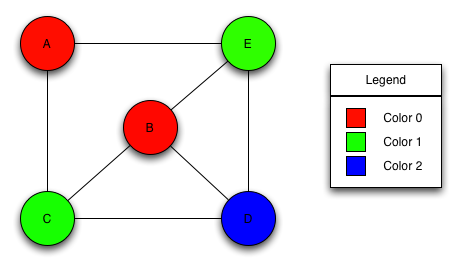
\includegraphics[scale=1]{figures/graph-sol.png}
	\caption{Lời giải của bài toán tô màu đồ thị\label{fig:graphSol}}
\end{figure}

Bài toán tô màu đồ thị yêu cầu tô màu cho các đỉnh của đồ thị sao cho không có hai đỉnh liền kề nhau có cùng màu.

Mô hình toán học:

Đồ thị $G(V,E), K$ màu cho trước \nocite{b2d1}.
\begin{itemize}
	\item $X = \{X_i | 1 \leq i \leq |V|\}$ \quad là các màu tô trên các đỉnh của đồ thị.
	\item $D = \{D_i | 1 \leq i \leq |V|\}$ \quad là miền giá trị cho các $X_i$, $D_i = \{1,\dots,K\}$
	\item Tập ràng buộc $C$:
	$X_i \neq X_j$ nếu \exists $e \in E, e = (V_i, V_j)$
	\item Hàm mục tiêu:
	Cực tiểu số lượng màu cần phải tô tren đồ thị $G(V,E)$ 
\end{itemize}

Hình \ref{fig:graphSol} là một lời giải cho bài toán tô màu đồ thị.

%----------------------------------------------------------------
\subsection{Một số kỹ thuật giải bài toán tối ưu tổ hợp}
\subsubsection*{Quy hoạch ràng buộc \cite{rossi2006handbookOfCp, pascal2005cp}}
Là kỹ thuật cơ bản để giải quyết bài toán thỏa mãn ràng buộc, mô hình của kỹ thuật quy hoạch ràng buộc như sau: 
\[ CP = Model + Search\]
Trong đó:
\begin{itemize}
	\item \textsc{Model} là tập các biến, miền giá trị và ràng buộc của bài toán.
	\item \textsc{Search} là thủ tục tìm kiếm lời giải dựa trên các ràng buộc, thủ tục này có thể là các thuật toán tìm kiếm theo chiều rộng, tìm kiếm theo chiều sâu\dots và có sử dụng các kỹ thuật cắt tỉa phù hợp làm giảm không gian tìm kiếm.
\end{itemize}

Cụ thể các bước thực hiện như sau:
\begin{itemize}
	\item Khởi tạo mô hình tìm kiếm, không cần thiết phải khởi tạo giá trị cho các biến bộ phận.
	\item Trong mỗi bước lặp, các biến bộ phận được lần lượt gán giá trị trong các thủ tục đệ quy, thủ tục này sẽ đệ quy cho đến khi tất cả các biến bộ phận được gán đầy đủ giá trị phù hợp với ràng buộc của bài toán và sẽ quay lui khi tìm được một phương án hoặc là phát hiện ra hướng tiếp theo không có phương án nào phù hợp.
\end{itemize}
Kỹ thuật này có ưu điểm dễ cài đặt, ý tưởng trong sáng tuy nhiên khi gặp bài toán có không gian lời giải lớn và rất lớn thì nó tỏ ra không hiệu quả khi không thể đưa ra được một phương án dù đó là phương án tồi vì nó yêu cầu duyệt gần như toàn bộ không gian lời giải.
\subsubsection*{Tìm kiếm cục bộ \cite{dungpq2015cbls}}
Là kỹ thuật tìm kiếm lời giải dựa trên việc lặp đi lặp lại thao tác lựa chọn lời giải có chất lượng tốt hơn trong không gian lời giải lân cận, phương pháp này có nhiều ưu điểm hơn trong những bài toán có không gian tìm kiếm lớn, cụ thể về phương pháp này tôi xin trình bày ở mục tiếp theo.
%====================================================================
\section{Tìm kiếm cục bộ dựa trên ràng buộc}
Với các bài toán tối ưu tổ hợp chúng ta luôn phải làm việc với các bộ giá trị gán cho các biến để tìm ra bộ giá trị đảm bảo thỏa mãn các ràng buộc và tối ưu hóa hàm mục tiêu. Số lượng các tập có thể của các bộ này rất lớn nên chúng ta khó có thể đưa ra một giải thuật hiệu quả để duyệt hết phương án cũng như khó có thể đưa ra một giải thuật cắt tỉa phù hợp để loại bỏ các nhánh không cần thiết.

Tiếp cận theo hướng tìm kiếm cục bộ giảm được các khó khăn nêu trên, nó không yêu cầu nhiều bộ nhớ, không yêu cầu quá nhiều thời gian tính toán. Trong tìm kiếm cục bộ ta sử dụng một số khái niệm:
\begin{itemize}
	\item \textbf{Láng giềng} của một phương án $S$ là các phương án $\{S_1, S_2,\dots, S_m\}$ được sinh ra từ $S$ bằng cách thay đổi một vài giá trị bộ phận trong phương án của $S$.
	\item \textbf{Cực tiểu địa phương} là phương án thỏa mãn các ràng buộc và có giá trị hàm mục tiêu nhỏ hơn so với các láng giềng quanh nó.
\end{itemize}

Với phương pháp tìm kiếm cục bộ, chúng ta không phải duyệt hết tất cả các bộ tổ hợp của bài toán mà thay vào đó sẽ tìm kiếm các phương án địa phương thỏa mãn các ràng buộc và cực tiểu hóa hàm mục tiêu. Từ các phương án địa phương này ta sẽ lần lượt đi đến các phương án địa phương khác tốt hơn và tiếp tục cho đến khi ta có một phương án mới là phương án tối ưu toàn cục. Sau một số bước nhất định việc tìm kiếm cục bộ sẽ đưa chúng ta đến phương án cục bộ mới tốt hơn và có thể đến được phương án tối ưu hoặc là phương án gần tối ưu mà chúng ta coi nó là chấp nhận được với yêu cầu bài toán.

Các bước của một giải thuật tìm kiếm cục bộ như sau:
\begin{itemize}
	\item \textsc{Khởi tạo:} Sinh lời giải xuất phát $s$, tính toán các vi phạm ràng buộc, hàm mục tiêu.
	\item \textsc{Tìm kiếm lân cận:} từ lời giải hiện tại, giải thuật sinh ra tập lời giải láng giềng bằng \[S = N(s)\]cách thay đổi một vài thành phần của phương án hiện tại. Từ tập lời giải mới này ta cần tìm ra phương án $s'$ có chất lượng tốt nhất.
	\item \textsc{Di chuyển:} sau khi tìm được phương án mới có chất lượng tốt, ta thực hiện di chuyển lời giải sang phương án mới này và cập nhật lại giá trị vi phạm và hàm mục tiêu.
	\item \textsc{Kiểm tra:} kiểm tra các điều kiện dừng, nếu thỏa mãn thì kết thúc tìm kiếm, nếu không sẽ thực hiện quay lại bước \textsc{Tìm kiếm lân cận}.
\end{itemize}

Các giải thuật tìm kiếm cục bộ được cải thiện đáng kể nhờ sử dụng các Heuristic để tăng cường chất lượng các lời giải láng giềng.

Giải thuật tìm kiếm cục bộ sử dụng một số phương pháp tìm kiếm sau:
\begin{itemize}
	\item Kỹ thuật leo đồi \cite{rossi2006handbookOfCp} lời giải được bắt đầu từ một vị trí ngẫu nhiên và quan sát xung quanh để xem phương án nào tốt hơn quanh nó để đi đến, sau một số lần lặp, nó sẽ đưa đến một phương án tối ưu địa phương.
	\item Kỹ thuật tìm kiếm tabu \cite{rossi2006handbookOfCp} trong bước dịch chuyển của thuật toán tìm kiếm cục bộ, một phương án được phép dịch chuyển nếu như nó hoàn toàn không bị cấm. Một phương án bị cấm là phương án đã được dịch chuyển đến trước đó. Nhờ sử dụng kỹ thuật này chúng ta giảm được sự tìm kiếm xoay vòng quanh các phương án trước đó.
\end{itemize}


%------------------------------------------------------------------
\section{Thư viện JOpenCBLS}
\subsection{Tổng quan}
JOpenCBLS là bộ thư viện được viết bằng ngôn ngữ JAVA do TS. Phạm Quang Dũng và các thành viên Lab \textsf{thuật toán và tối ưu - Viện Công nghệ thông tin truyền thông, đại học Bách Khoa Hà Nội} thiết kế và cài đặt.

Thư viện góp phần giảm công sức trong việc giải các bài toán tối ưu thỏa mãn ràng buộc bằng phương pháp tìm kiếm cục bộ. Để sử dụng hiệu quả thư viện người dùng cần biểu diễn miền giá trị, biểu diễn lời giải và các ràng buộc thích hợp. Dựa vào các thông tin được cung cấp sẵn thư viện sẽ tự động thực hiện công việc tìm kiếm kết quả theo phương pháp \textsf{tìm kiếm cục bộ}. Kiến trúc của thư viện JOpenCBLS dựa trên kiến trúc của \textsf{Constraint-based Local Search - CBLS} - \textsf{Van Hentenryck \& Michel 2005}. Thư viện được thiết kế và cài đặt trên ngôn ngữ JAVA do đó thư viện có được tính linh hoạt, tùy biến mở rộng và tái sử dụng của nền tảng JAVA. Điều đó giúp cho JOpenCBLS đã sẽ và đang góp phần rất tích cực trong quá trình giảng dạy, học tập và nghiên cứu của các cán bộ, sinh viên viện công nghệ thông tin trong Viện công nghệ thông tin - đại học Bách Khoa.

JOpenCBLS hướng đến việc đơn giản hóa các công việc xây dựng chương trình, cấu trúc dữ liệu và thiết kế thuật toán với bộ các thuật toán được cài đặt sẵn trong thư viện. Nó giúp cho người sử dụng có thêm thời gian tập trung nghiên cứu biểu diễn dữ liệu, mô hình hóa các ràng buộc của bài toán, cài đặt thử nghiệm các chiến lược tìm kiếm \textsc{heuristic} và \textsc{meta heuristic} để giải quyết bài toán.

Cấu trúc thư viện JOpenCBLS:
\begin{itemize}
	\item Mô hình (Model) nhằm mô hình hóa các bài toán, biểu diễn chúng để sau đó có thể thực hiện quá trình tìm kiếm:
	\begin{itemize}
		\item Các biến.
		\item Các đại lượng bất biến.
		\item Các hàm.
		\item Các ràng buộc.
	\end{itemize}
	\item Tìm kiếm (Search) chứa các thủ tục tìm kiếm được cài đặt sẵn với các giải thuật:
	\begin{itemize}
		\item Tabu Search.
		\item SA Search.
	\end{itemize}
\end{itemize}

%-------------------------------------------------------------------------------------------
\subsection{Các thành phần của JOpenCBLS}

\subsubsection{Mô hình}
\textbf{Biến (Variable)}
\begin{itemize}
	\item Biến trong JOpenCBLS là một đối tượng JAVA dùng để biểu diễn một bộ phận của phương án trong quá trình tìm kiếm, tập các biến cho ta một phương án.
	\item JOpenCBLS có 2 lớp cơ bản biểu diễn biến là \textsf{VarInt} và \textsf{VarIntLS}, trong đó \textsf{VarInt} là lớp biểu diễn cơ bản cho một biến, lớp \textsf{VarIntLS} kế thừa \textsf{VarInt} và cài đặt thêm các phương thức để thao tác trong quá trình tìm kiếm.
\end{itemize}

\textbf{Bất Biến (Invariants)}
\begin{itemize}
	\item Đại lượng bất biến là các đối tượng JAVA lưu giữ mối quan hệ giữa các biến, miền giá trị, mối quan hệ giữa biến và ràng buộc. Đại lượng này không thay đổi trong quá trình thực hiện tìm kiếm lời giải.
	\item Trong JOpenCBLS, \textsf{Invariant} là một \textit{interface}, nó cần được cài đặt lại khi cần thể hiện ràng buộc giữa các biến.
\end{itemize}

\textbf{Hàm (Functions)}
\begin{itemize}
	\item Là các đối tượng biểu diễn các hàm thay đổi giá trị được phụ thuộc vào giá trị các biến trong mô hình.
\end{itemize}

\textbf{Ràng buộc (Constraints)}
\begin{itemize}
	\item Là các đối tượng JAVA biểu diễn ràng buộc của bài toán, cũng giống như các hàm, nó thay đổi được giá trị và phụ thuộc vào giá trị các biến.
\end{itemize}

\subsubsection{Tìm kiếm (Search)}
JOpenCBLS có sẵn các phương thức để thao tác với biến trong quá trình tìm kiếm trong lớp \textsf{MinMaxSelector}:
\begin{itemize}
	\item \textit{MinMaxSelector(IConstraint s)}\\ là hàm khởi tạo đối tượng lựa chọn trong mô hình gắn với hệ thống ràng buộc s.
	\item \textit{selectMostViolatedVariable()}\\ là hàm trả về đối tượng biến trong mô hình có số lượng ràng buộc bị vi phạm liên quan đến nó nhiều nhất.
	\item \textit{selectMostPromissingValue(VarIntLS x)}\\ trả về giá trị làm giảm số lượng vi phạm nhiều nhất trong với biến x.
\end{itemize}

JOpenCBLS cũng đã cài đặt các kỹ thuật tìm kiếm trong lớp \textsf{TabuSearch} để giải quyết các bài toán với các thủ tục tìm kiếm tabu như:
\begin{itemize}
	\item \textit{search(s, tabuLength, maxTime, maxIter, maxStable)}\\
	Tìm kiếm với tabu heuristic nhận tham số đầu vào:
	\begin{itemize}
		\item \textit{s} Hệ thống ràng buộc.
		\item \textit{tabuLength} số bước lặp bị cấm với cùng một thao tác dịch chuyển láng giềng.
		\item \textit{maxTime} thời gian chay tối đa (tính theo giây) của thủ tục tìm kiếm tabu này.
		\item \textit{maxIter} số vòng lặp (láng giềng) tối đa trong quá trình tìm kiếm.
		\item \textit{maxStable} số lượng tối đa các láng giềng đi qua nếu không tìm thấy sự cải thiện hàm mục tiêu.
	\end{itemize}	
	\item \textit{searchAssignSwap(s, tabuLength, maxIter, maxTime)}\\
	Tìm kiếm tabu bằng cách xem xét cả việc gán giá trị cho các biến và tráo đổi giá trị từng cặp biến với nhau, nhận tham số đầu vào:
	\begin{itemize}
		\item \textit{s} hệ thống ràng buộc.
		\item \textit{tabuLength} số bước bị cấm dịch chuyển sau khi thực hiện dịch chuyển đó.
		\item \textit{maxIter} số bước lặp tối đa.
		\item \textit{maxTime} thời gian tối đa thực hiện tìm kiếm.
	\end{itemize}	
	\item \textit{searchMaintainConstraint(f, s, maxTime, maxIter, maxStable)}\\
	Tìm kiếm tabu thực hiện thỏa mãn tất cả ràng buộc trong s và cực tiểu hóa hàm mục tiêu f, nhận tham số đầu vào:
	\begin{itemize}
		\item \textit{f} hàm mục tiêu cần cực tiểu hóa.
		\item \textit{s} hệ thống ràng buộc.
		\item \textit{maxTime}  thời gian chạy tối đa của thủ tục tìm kiếm.
		\item \textit{maxIter} số lượng bước lặp tối đa.
		\item \textit{maxStable} số lần lặp tối đa để khởi động lại lời giải.
	\end{itemize}	 
\end{itemize}

\subsubsection{Ví dụ minh họa}
Dưới đây là một ví dụ minh họa việc cài đặt bài toán N-QUEENS sử dụng JOpenCBLS:
\begin{itemize}
	\item \textbf{Mô hình bài toán}
	\begin{lstlisting}
		//NQueen.java

		...		
		
		int n = 10000;
		
		LocalSearchManager ls = new LocalSearchManager();
		VarIntLS[] x = new VarIntLS[n];
		
		for (int i = 0; i < n; i++){
			x[i] = new VarIntLS(ls, 0, n - 1);
			
		ConstraintSystem s = new ConstraintSystem(ls);
		s.post(new AllDifferent(x));
		
		IFunction[] f1 = new IFunction[n];
		for (int i = 0; i < n; i++)
			f1[i] = new FuncPlus(x[i], i);
		s.post(new AllDifferent(f1));
		
		IFunction[] f2 = new IFunction[n];
		for (int i = 0; i < n; i++)
			f2[i] = new FuncPlus(x[i], -i);
		s.post(new AllDifferent(f2));
		
		ls.close();		
		...
	\end{lstlisting}
	Để thực hiện khởi tạo chúng ta cần khai báo một \textsf{LocalSearchManager} quả lý tất cả các biến, sau đó khai báo các biến trong mô hình và khởi tạo nó. Tiếp theo chúng ta cần có một hệ thống ràng buộc và thực hiện lưu giữ các ràng buộc lại trong hệ thống ràng buộc $s$. Ở đây, với bài toán n-queens chúng ta có 3 ràng buộc cơ bản:
	\begin{itemize}
		\item các quân hậu không cùng nằm trên cùng một cột,
		\item các quân hậu không cùng nằm trên cùng một đường chéo thuận,
		\item các quân hậu không cùng nằm trên cùng một đường chéo ngược. 
	\end{itemize}
	Sau khi khởi tạo các biến, mô hình và tải các ràng buộc, chúng ta cần đóng mô hình để thư viện thực hiện các thủ tục khởi tạo, cập nhật hệ thống ràng buộc cần thiết.
	\item \textbf{Thực hiện tìm kiếm}
	\begin{lstlisting}
		//NQueen.java
		MinMaxSelector mms = new MinMaxSelector(s);
		int it = 0;
		while(it < 10000 && s.violations() > 0){
			VarIntLS variable = mms.selectMostViolatedVariable();
			int selectValue = mms.selectMostPromissingValue(variable);
			variable.setValuePropagate(selectValue);
			it++;
		}
		System.out.println("Current violations: " + s.violation());
	\end{lstlisting}
	Với đoạn mã thực hiện việc tìm kiếm này chúng ta có một đối tượng lựa chọn để lấy các thông tin, các đối tượng mà chúng ta yêu cầu sau đó tiếp tục thực hiện gán giá trị cho các biến chúng ta lấy được. Cụ thể ở đây ta luôn chọn đối tượng biến có số lượng vi phạm có liên quan đến nó là nhiều nhất sau đó gán cho nó giá trị mới sao cho số lượng vi phảm được giảm đi cũng là nhiều nhất, tiếp tục lặp thao tác vừa rồi cho tới khi không còn vi phạm hoặc số vòng lặp vượt quá tối đa. Kết thúc vòng lặp chúng ta có kết quả của thủ tục tìm kiếm này.
\end{itemize}

%============================================================================================
%\section{Kết luận}
%Các bài toán tối ưu tổ hợp rất phổ biến trong cuộc sống và cũng là những vấn đề lớn cần giải quyết song không phải dễ dàng giải quyết chúng, công việc giải quyết đòi hỏi rất nhiều thời gian và công sức.

%Tìm kiếm cục bộ dựa trên ràng buộc là phương pháp khả thi hơn cả và với thư viện JOpenCBLS của tiến sỹ Phạm Quang Dũng chúng ta có một bộ công cụ đủ mạnh để thực hiện các bài toán này. Trong phần tiếp theo tôi sẽ đi sâu phân tích, mô hình và giải quyết một bài toán trong số các bài toán tối ưu này đó là bài toán \textsc{đóng thùng} (Bin Packing) ở mức 2 chiều.
